% Source: HowToTex.com
\documentclass{article}
\usepackage{booktabs}
\usepackage{caption}
\usepackage{geometry}
\usepackage{fancyhdr}
\pagestyle{fancy}
\fancyhf{}
\fancyhead[R]{\textcolor{gray}{Mock Draft}}
\fancyfoot[C]{\thepage}
\rhead{CP 213 \\ December 9, 2016}
\lhead{Brian Goggin}


%~~~~~~~~~~~~~~~~~~~%

\input /Users/briangoggin/Dropbox/CP_213/Paper/maitaCustomCommands.tex
\usepackage[T1]{fontenc} % Use 8-bit encoding that has 256 glyphs
\usepackage{fourier} % Use the Adobe Utopia font for the document - comment this line to return to the LaTeX default
\usepackage[english]{babel} % English language/hyphenation
\usepackage{amsmath,amsfonts,amsthm} % Math packages
\usepackage{enumerate}
\usepackage{graphicx, here}
\usepackage{caption,subcaption}
\usepackage{color,soul}
\usepackage{amssymb}
\usepackage{amsmath}
%\captionsetup[figure]{labelfont={bf},name={Figure},labelsep=period} % use to bold figure title
\usepackage[format=hang,font=normalsize,labelfont=bf]{caption} % use to bold table and figure titles
\usepackage{ctable}  %use for thick horizontal lines in table
\usepackage{hyperref} %used to make interactive links to web links
\usepackage[hang,flushmargin]{footmisc} 





%----------------------------------------------------------------------------------------
%	TITLE SECTION
%----------------------------------------------------------------------------------------

\newcommand{\horrule}[1]{\rule{\linewidth}{#1}} % Create horizontal rule command with 1 argument of height

\title{	
\normalfont \normalsize 
\textsc{University of California, Department of City \& Regional Planning} \\ [25pt] % Your university, school and/or department name(s)
\horrule{0.5pt} \\[0.4cm] % Thin top horizontal rule
\huge CP 213 Case Study: Evaluating Fruitvale TOD's Impacts on Transit Ridership \\ % The assignment title
\horrule{2pt} \\[0.5cm] % Thick bottom horizontal rule
}

\author{Brian Goggin} % Your name

\date{\normalsize\today} % Today's date or a custom date






%~~~~~~~~~~~~~~~~%
\begin{document}

\maketitle % Print the title
\newpage



\section*{1 Background: Fruitvale Transit Village}

Completed in 2004, the Fruitvale Transit Village---a transit-oriented development (TOD)---has been praised as a much-needed economic stimulus for an underprivileged community. In this case study, I explore the impacts of the project on transit ridership---which surveys have found is the most commonly cited motivation of transit agencies for TODs (Cervero et al. 2004, 9). In the next section, I discuss the motivations behind the project and the changes that planners made to increase transit ridership. In the following section, I examine ridership changes at the Fruitvale BART station before and after the transit village. 

\subsection*{1.1 Project  Motivations}

During the project, BART worked with a local community development corporation known as the Unity Council to better connect the Fruitvale BART station with the surrounding community. While the Unity Council emphasized local pollution reduction and economic development, BART was interested in the potential for ridership increases (FHWA 2015). In particular, BART expected that the development would add from 300 to 600 new daily riders at the Fruitvale station. (FHWA 2015).  \\

\noindent
Eventually, the Fruitvale Transit Village Phase I took shape with three major pieces---a large mixed-use development adjacent to the station, a new multi-level BART parking garage, and new pedestrian corridor connecting the station to Fruitvale. In the remainder of this section, I will describe these three project components in more detail with their intended effects on transit ridership. \\

\subsection*{1.2 Land Use Changes}

BART and the Unity Council both agreed that the primary improvement to the transit station was to replace a 9-acre surface parking lot with mixed-use development (FHWA 2015). This parking lot presented major obstacles for community residents to walk or bike to the station. Furthermore, riders exiting the Fruitvale station were disconnected from the main Fruitvale commercial corridor on International Boulevard and were only able to see the backs of building in the distance. In order to improve this, the project arranged for two new developments---a major mixed-use development on the site of the former parking lot and a replacement multi-level parking garage to the south of the station (FHWA 2015). To tie the project in with the adjacent International Boulevard and BART station, leaders planned for a pedestrian corridor through the heart of the development. Figures 1 and 2 below illustrate these changes.  \\

\noindent
The City of Oakland aided the project by creating a transit-oriented overlay zone (S15) on the former site of the parking lot. This allowed for high-density, mixed-use development (Scully 2005). While phase I of the transit village only has 47 residential units, it also includes 40,000 square feet of ground-floor retail space and 114,509 square feet of office space (Scully 2005). These spaces include community social services and gathering places, such as a library, pre-k education, a health care center, and a grocery store (Unity Council 2016). Ultimately BART hoped that this development would provide activity centers around the transit station to encourage more transit usage. \\

\newpage

\begin{figure}[H]
	\label{fig:Figure 1}
	\caption{\textbf{Fruitvale Transit Station Before TOD}}
	\begin{minipage}{\textwidth} % choose width suitably
	\includegraphics[width=\linewidth]{pre_TOD_map.jpg}
	{\footnotesize Source: UC Berkeley Earth Sciences and Map Library. 1994 Oakland, CA Digital Geographic System, Inc. in association with WAC Corporation. NAD 1983 State Plane California (3) Projection.\par}
\end{minipage}
\end{figure}

\begin{figure}[H]
	\label{fig:Figure 2}
	\caption{\textbf{Fruitvale Transit Station After TOD}}
	\begin{minipage}{\textwidth} % choose width suitably
	\includegraphics[width=\linewidth]{post_TOD_map.jpg}
	{\footnotesize Source: Image from April 2005 captured from Google Earth. NAD 1983 State Plane California (3) Projection.\par}
	\end{minipage}
\end{figure}


\subsection*{1.3 Parking Changes}

BART required that the Unity Council replace all lost space from the surface lot. As a result, the project built a new multi-layered parking facility consisting of 558 spaces south of the BART tracks (Bigelow 2014, 18).  Aside from BART, there was also community support for retaining parking spaces, particularly from concerned merchants along International Boulevard. To address this concern, the transit village\textquotesingle s phase I development provides additional at-grade covered parking for 150 cars (Scully 2005). As a result, the transit village actually resulted in a net increase in parking.  \\

\subsection*{1.4 Design Changes}

Along with the land use and parking alterations, the Unity Council gave substantial attention to the design of the new pedestrian spaces. In order to create appeal for passer-byes, the mixed-use buildings have all retail space on the bottom, followed by office space in the middle and residential units on the top floors (Scully 2005). Furthermore, the architectural style blended Mediterranean and Mexican styles with a light color palate, hoping to achieve a festive atmosphere while also representing the culture of the area (Scully 2005). Figure 3 below is a picture of the development that captures the pedestrian\textquotesingle s point of view. \\

\begin{figure}[H]
	\label{fig:Figure 3}
	\caption{\textbf{Fruitvale Transit Village Pedestrian Corridor}}
	\centering
	\begin{center}
	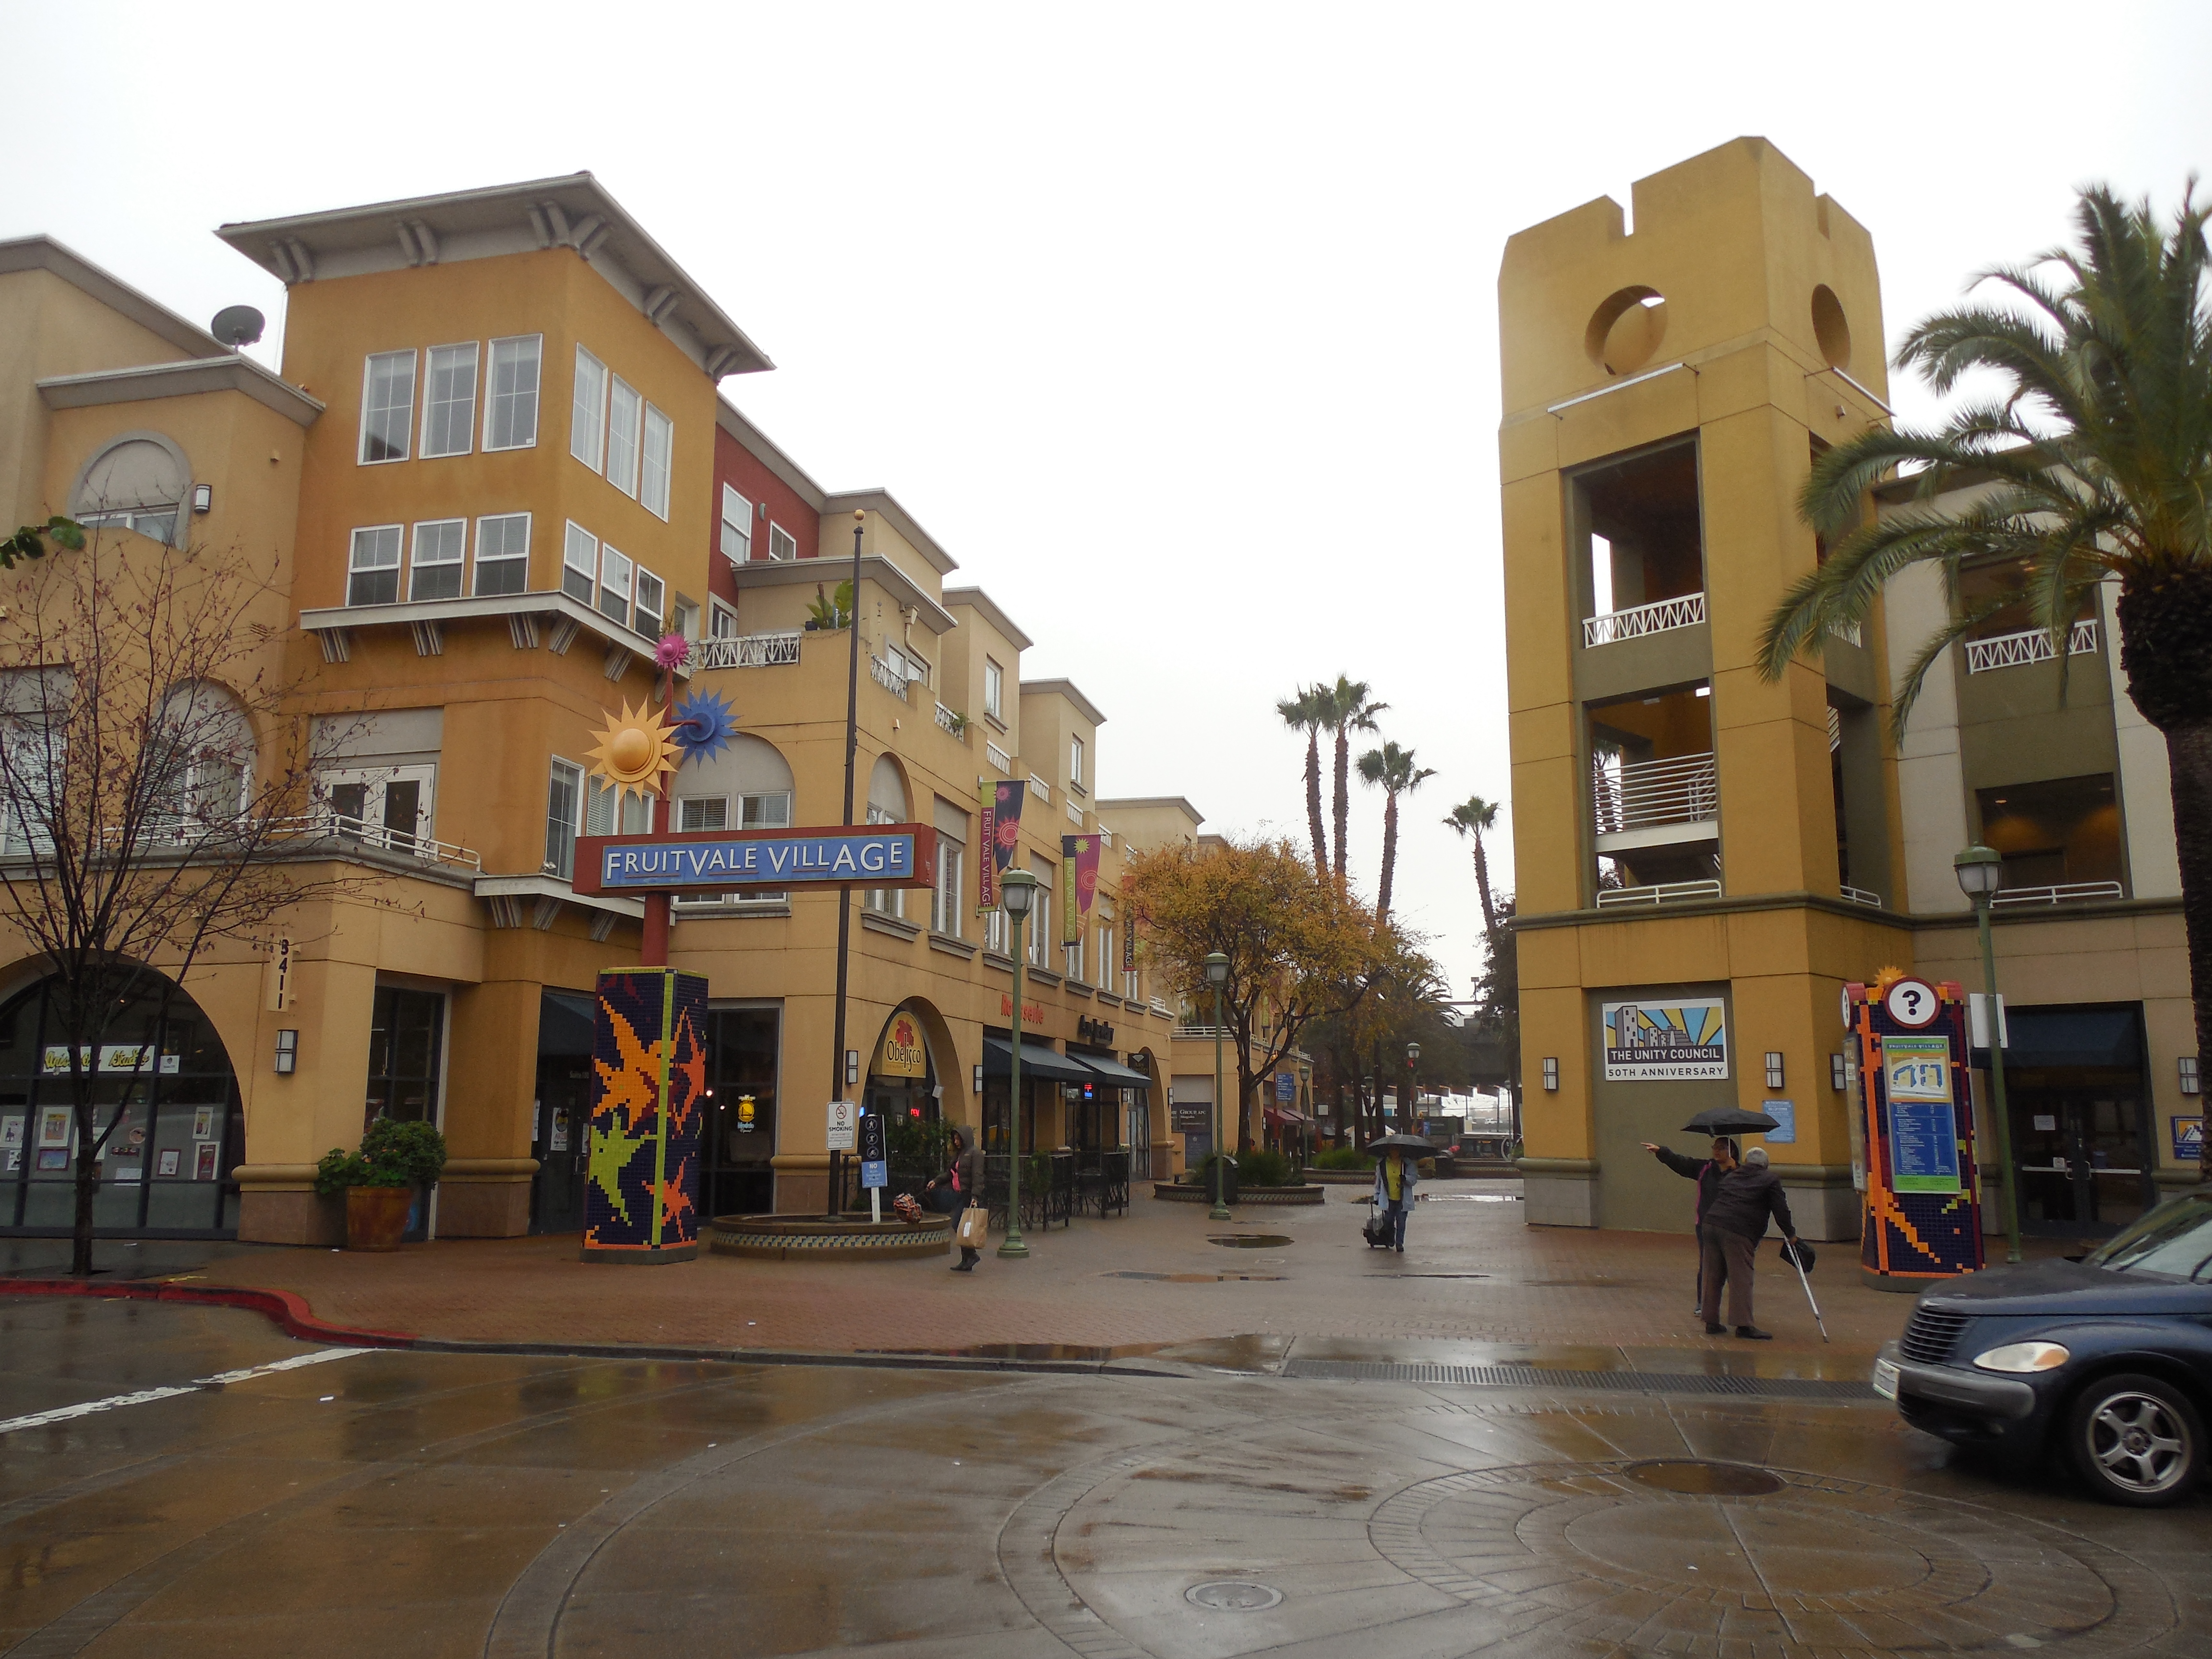
\includegraphics[width=0.9\linewidth]{fig3.jpg} 
	\end{center}
	\begin{minipage}{0.9\linewidth}
		{\par \footnotesize This picture shows the festive design elements of the pedestrian corridor. Picture taken facing the BART tracks, which can be seen in the back. Picture taken on December 8, 2016.\par}
	\end{minipage}
\end{figure}

\noindent
Despite these efforts, there were numerous reasons for concern that these design changes would not stimulate increases in ridership. Although community planners put tremendous effort into the central pedestrian corridor, the backsides of the transit village went neglected with little-to-no activity. Figure 4 illustrates this below (Bigelow 2014, 12). \\

\begin{figure}[H]
	\label{fig:Figure 4}
	\caption{\textbf{Backside of Fruitvale Transit Village}}
	\centering
	\begin{center}
	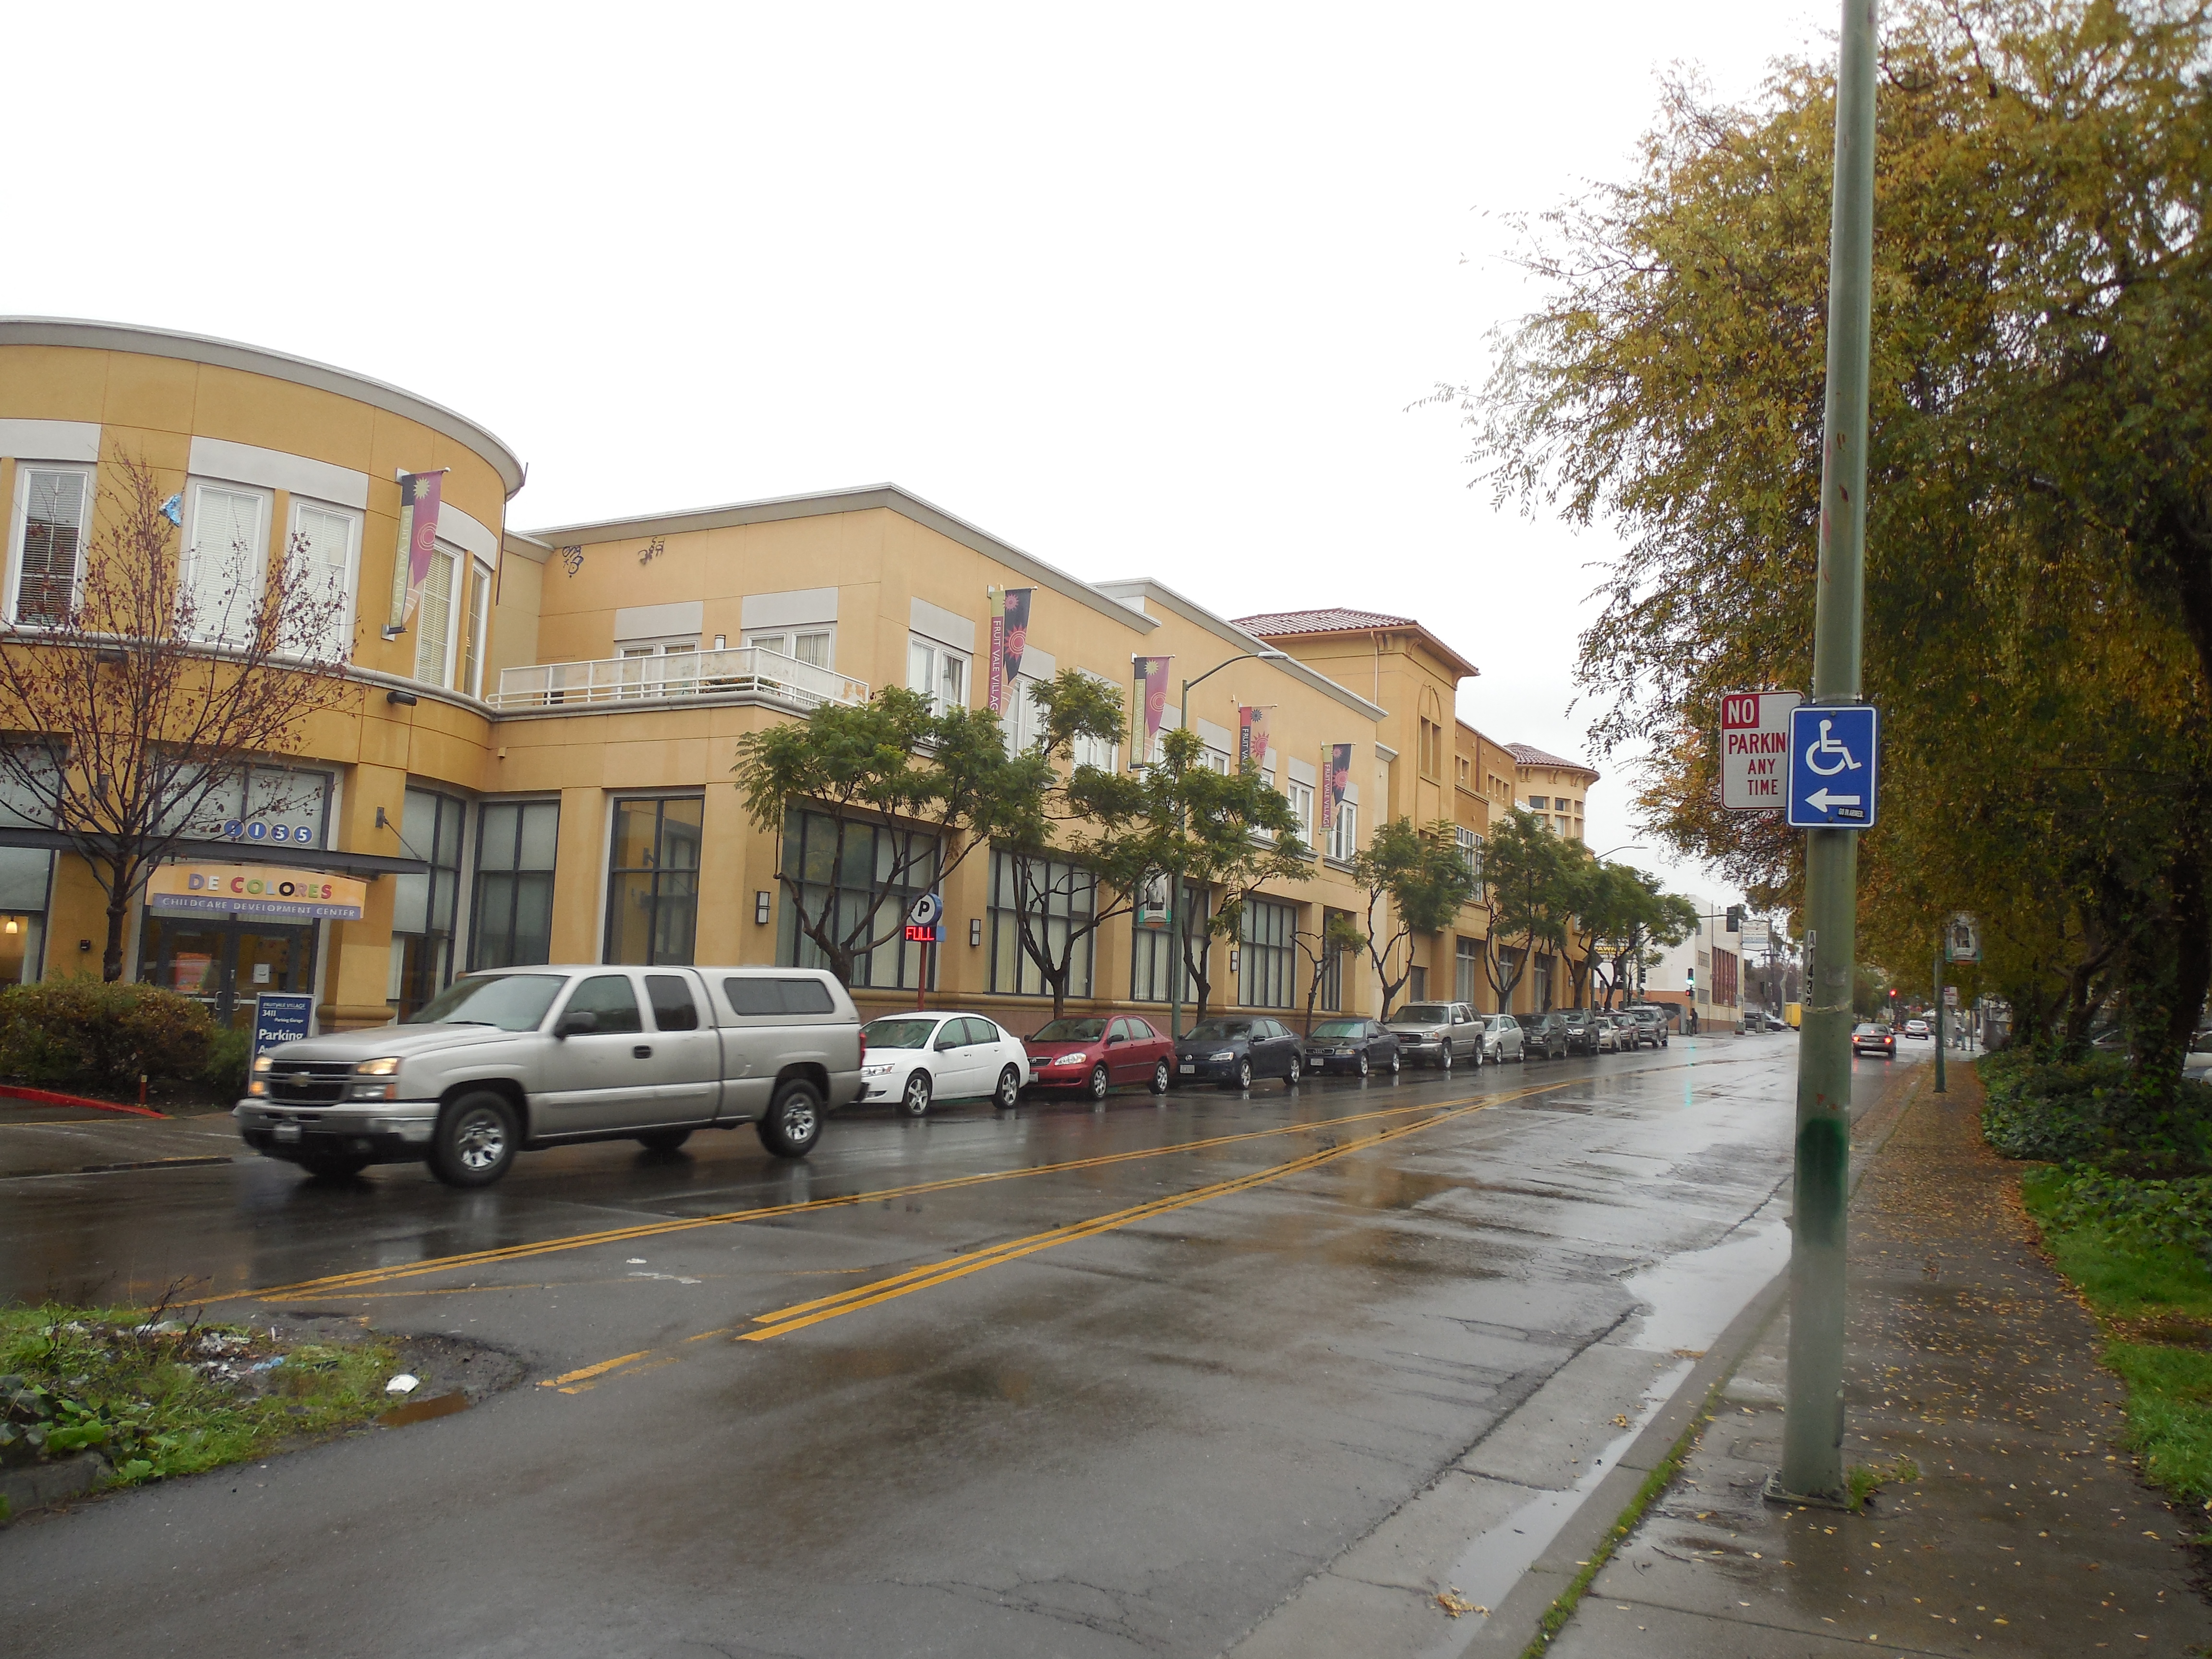
\includegraphics[width=0.9\linewidth]{fig4.jpg}
	\end{center}
	\begin{minipage}{0.9\linewidth}
	{\par \footnotesize This picture shows the activity-less backside of the transit village on an adjacent street. Picture taken on December 8, 2016.\par}
	\end{minipage}
\end{figure}

\noindent
Furthermore, community leaders pushed for restricting the heights of the buildings to keep them in line with the neighborhood scale. This was despite the fact that the new zoning would have allowed them to go higher, presumably enabling more residential units (Scully 2005). \\

\section*{2 Impacts on BART Ridership}

\subsection*{2.1 Theory on Potential Impacts}

The increased activity around the BART station probably draws more people to the area, but these additional people will not necessarily come by transit. In surveys of transit agencies across the U.S., Cervero et al. (2004) find that practitioners generally agree on some key elements of TOD---dense, diverse, and pedestrian-friendly---in order to increase transit usage. This development allows residences and activities to cluster close enough together so that residents do not rely on cars for daily activities. When they do need to travel longer distances, residents can use the transit close by. \\

\noindent
Academic studies have highlighted certain aspects of TOD that are key for inducing transit ridership over vehicle use. For example, Chatman (2013) found a strong positive influence of parking availability and strong negative influences of population and job density on automobile usage. Proximity to rail stations had no effect on vehicle usage independent of these forces. Moreover, Kamruzzaman et al. (2015) find crucial differences between TODs and poor imitations, or what they call transit-adjacent developments (TADs). These TADs are located near transit but have mostly homogenous land uses, poorly connected roads that inhibit walking, and low population densities. The authors found no transit ridership differences between these TADs and traditional suburbs. \\

\noindent
The Fruitvale Transit Village exhibits many of these crucial elements for increased transit usage, such as mixed uses, high population and job density, and walkability. However, there are some reasons for concern. The transit village has increased parking, and this presumably allows for many interested shoppers or residents to drive to the area instead of using transit. Moreover, the scale of the development was restricted due to community preferences, and this has likely limited the transit patronage increases. \\

\subsection*{2.2 Ridership Impacts}

In order to assess the effects of phase I of the transit village on ridership, I use station exit data from BART to compare Fruitvale station ridership before and after the project\textquotesingle s completion. First, Figure 5 shows the short-term ridership impacts---defined here as between the years 2001 and 2006. This graph compares the ridership increases at the Fruitvale BART station with the system-wide average. Despite there being increasing ridership after completion of the transit village, this trend is similar to the average station over the same time period. Next, Figure 6 shows a longer time horizon with annual averages. Due to data availability, I do not include data before 2001.\footnote{Station exit data comes from BART\textquotesingle s online ``Ridership Reports'' page, found at \url{http://www.bart.gov/about/reports/ridership}. Although station exits are available for 2000 and 1999, these are weekday exits only. I have decided to restrict the analysis to 2001-2016 because I can use a weighted average of weekday and weekend trips for these years.}  Despite an increasing annual trend after completion of the transit village in 2004, this also does not differ from the system-wide average. \\


\begin{figure}[H]
	\label{fig:Figure 5}
	\caption{\textbf{Monthly Average Daily Exits}}
	\begin{minipage}{\textwidth} % choose width suitably
	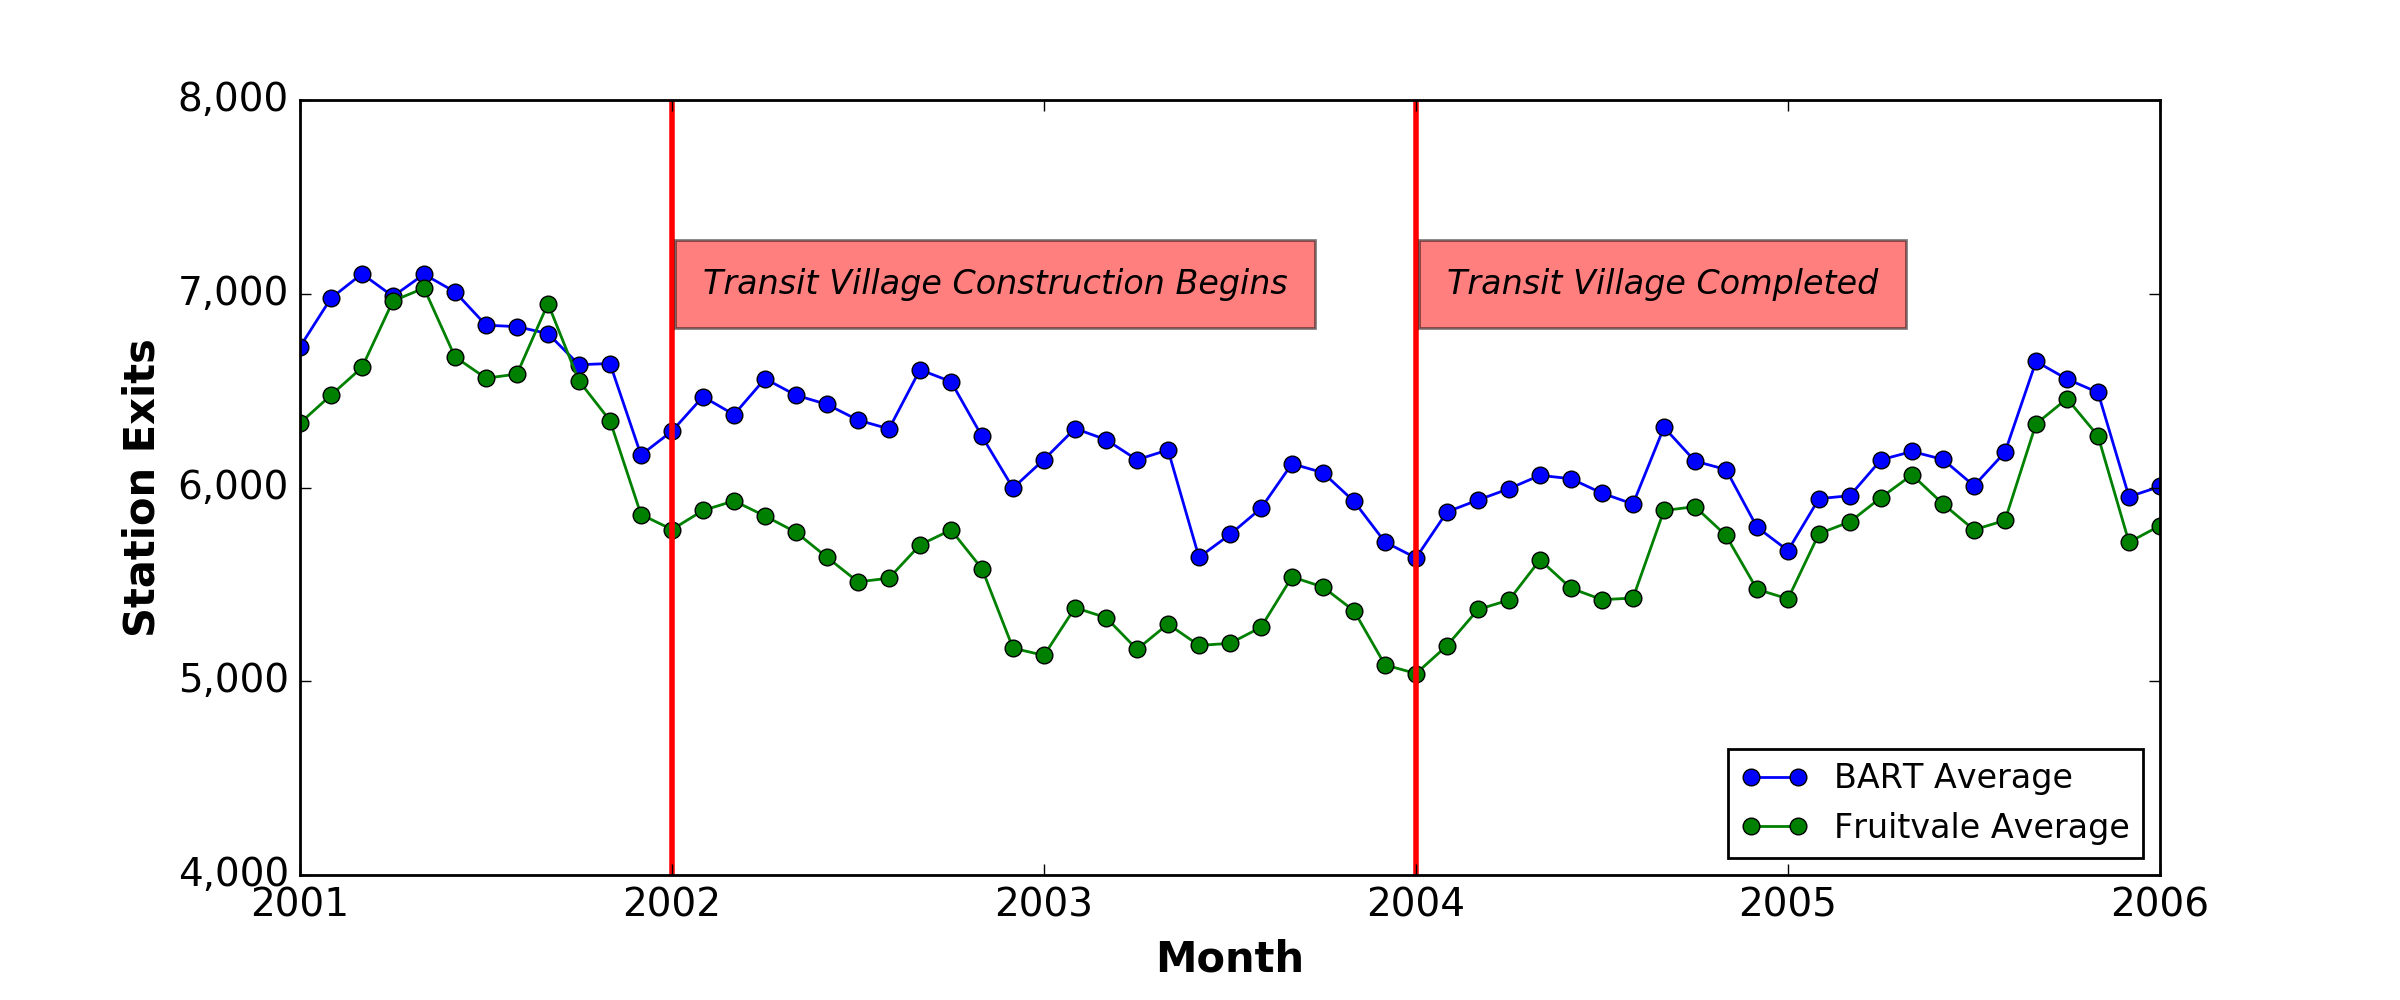
\includegraphics[width=\linewidth]{fig5.png}
	{\footnotesize Average daily exits are constructed from BART entry-exit data as a weighted average of weekday, Saturday, and Sunday exits.  \par}
	\end{minipage}
\end{figure}


\begin{figure}[H]
	\label{fig:Figure 6}
	\caption{\textbf{Annual Average Daily Exits}}
	\begin{minipage}{\textwidth} % choose width suitably
	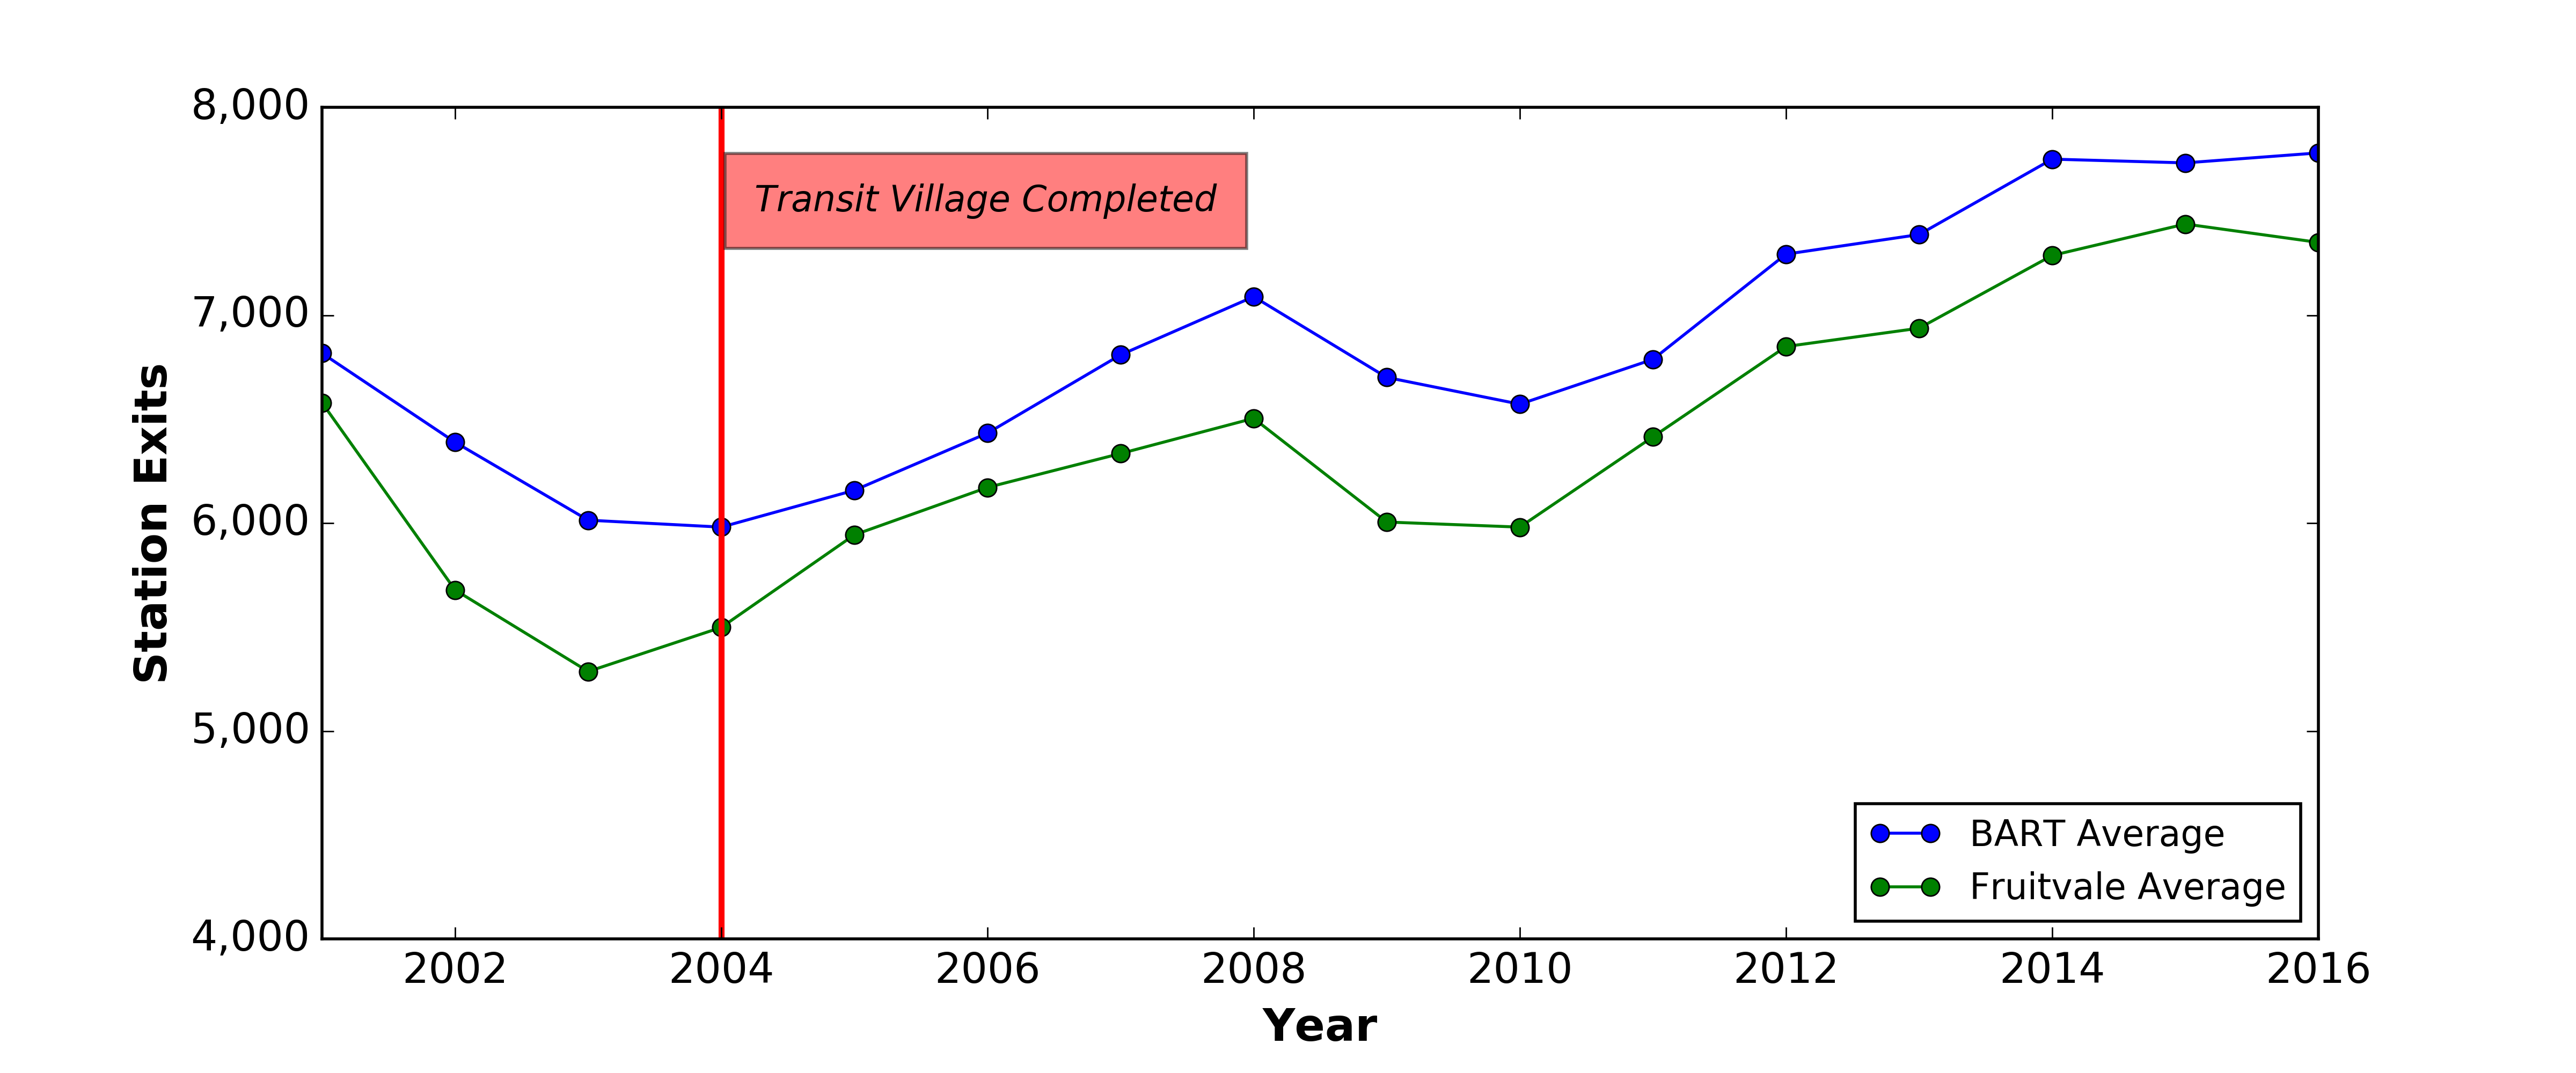
\includegraphics[width=\linewidth]{fig6.png}
	{\footnotesize Average daily exits are constructed from BART entry-exit data as a weighted average of weekday, Saturday, and Sunday exits.  \par}
	\end{minipage}
\end{figure}

\noindent
Finally, Figure 7 plots the difference between the two averages from 2001 to the present. The figure shows that Fruitvale station exits have remained fairly constant and below the system-wide average over time. I assess these differences with more precision in Table 1. This table shows that the Fruitvale Station did achieve BART\textquotesingle s goal of achieving a 300 to 600 increase in daily riders. However, the difference from the system-wide increase is only 116, which is well below the goal. \\

\begin{figure}[H]
	\label{fig:Figure 7}
	\caption{\textbf{Difference in Annual Average Daily Exits}}
	\begin{minipage}{\textwidth} % choose width suitably
	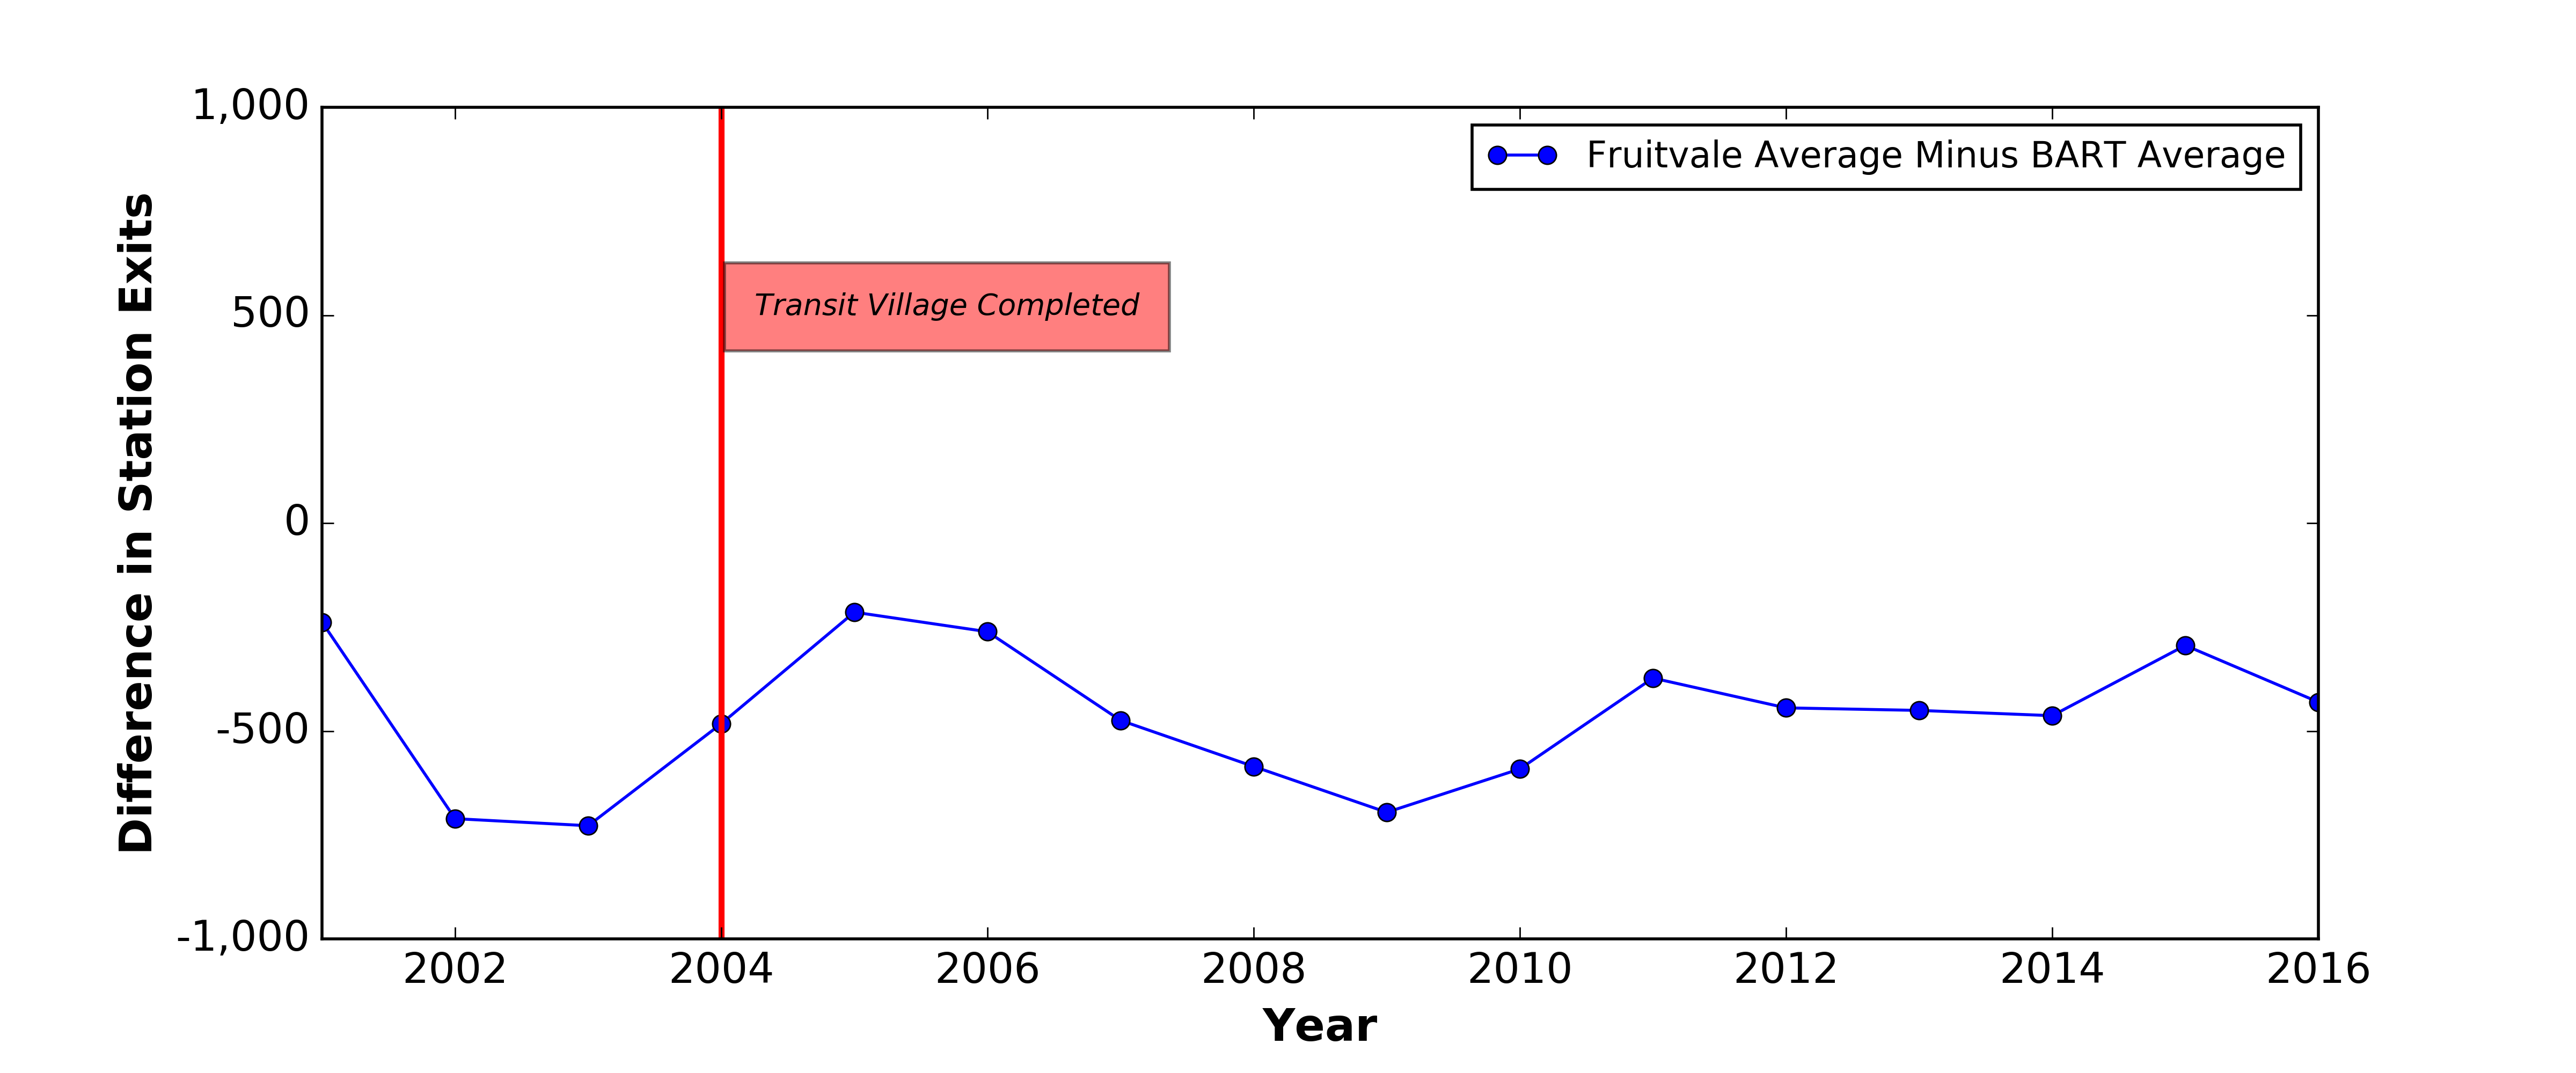
\includegraphics[width=\linewidth]{fig7.png}
		{\footnotesize Average daily exits are constructed from BART entry-exit data as a weighted average of weekday, Saturday, and Sunday exits.  \par}
	\end{minipage}
\end{figure}


\begin{table}[H]
\centering
\caption{\textbf{Average Daily Station Exits: Fruitvale Versus BART}}
\label{my-label}

\begin{tabular}{lcccc}
  \specialrule{.3em}{.2em}{.2em}
           & Pre Transit Village & Post Transit Village & Difference & Percentage Change \\
           \hline
Fruitvale  & 5,848               & 6,517                & 669        & 11\%              \\
BART       & 6,407               & 6,960                & 553        & 9\%               \\
\hline
Difference & -559                & -443                 & 116        & 2\%  \\
 \specialrule{.3em}{.2em}{.2em}           
\end{tabular}
\begin{minipage}{0.87\textwidth} % choose width suitably
{\footnotesize Note: The Fruitvale Transit Village Phase I was completed in 2004. Therefore, the pre-period is defined as the years 2001-2003 and the post-period is defined as the years 2004-2016. Average daily exits are constructed from BART entry-exit data as a weighted average of weekday, Saturday, and Sunday exits.  \par}
	\end{minipage}
\end{table}

\subsection*{2.3 Benefits Versus Costs}

The total cost for the Fruitvale Transit Village Phase I was approximately \$69 million (Scully 2005, 9). Of this, BART contributed a substantial amount through grants to construct the new parking facility (\$7.3 million), the new pedestrian corridor (\$780,000), and the new child care center (\$2.3 million) (FHWA 2015). Altogether this contribution amounts to approximately \$10.88 million, or about 16\% of the total. Assuming that BART\textquotesingle s sole motivation for the project was to increase revenue from ridership, a back-of-the-envelope calculation suggests that these project costs were not worth it.\\

\noindent
 Converting the project costs from 2004 to 2016 dollars, BART\textquotesingle s contribution amounts to \$13,794,388.\footnote{Conversion uses the CPI-U from the Minneapolis Federal Reserve. \url{https://www.minneapolisfed.org/community/teaching-aids/cpi-calculator-information/consumer-price-index-and-inflation-rates-1913}}  Next, assuming that each rider spends the average passenger fare and that there is an average increase of 669 daily riders via Table 1, the total increased fare revenues from the project are \$11,650,066.\footnote{The calculation uses the average passenger fare for 2016, \$3.67 (BART 2016), multiplies this by 365 for the days in a year, and then multiplies this by 13 for all the years between 2004 and 2016.}   Assuming BART could have used the grant money from the FTA for other projects, this represents a loss of over \$2 million.  Furthermore, this calculation was generous because I used 669 as the average daily increase in riders instead of 116, the difference from the system-wide average. Using this number instead, the increased fare revenue becomes  \$2,072,283, which amounts to a loss of over \$10 million dollars. This evidence suggests that the project was certainly not worth it if ridership was the primary concern. \\

\section*{3 Conclusion}

Yet, it would be difficult to call the Fruitvale Transit Village a failure. The development has added thousands of square feet of much-needed business and social services to a low-income community, all while retaining BART parking spaces. However, evaluating the project on the grounds of ridership increases---the top TOD priority for the majority of transit agencies---may be misguided. At best, ridership has only kept up with the larger system-wide trends, at a cost of millions of dollars. Instead, the success of the transit village stems from general densification, which replaced space-inefficient surface parking with a lively residential and commercial area. \\


\section*{4 References}

``BART 2016 Factsheet.'' 2016. BART. \url{https://www.bart.gov/sites/default/files/docs/2016Factsheet_v12.pdf} \\

\noindent
Bigelow, Justin. 2014. ``North Oakland Community Analysis.'' Transportation Studio, Fall 2014. Department of City and Regional Planning, UC Berkeley. \url{https://www.ocf.berkeley.edu/~abroaddu/wp-content/uploads/2015/01/FINAL-REPORT.pdf} \\

\noindent
Cervero, Robert, et al. 2004. Transit-Oriented Development in the United States: Experiences, Challenges, and Prospects. Chapter 1: Transit-Oriented Development: An Overview. Transit Cooperative Research Program. Transportation Research Board, National Research Council. \\

\noindent
Chatman, Daniel. 2013. ``Does TOD Need the T?'' Journal of the American Planning Association 79 (1): 17---31. \\

\noindent
``Fruitvale Transit Village Project - Case Studies - Environmental Justice - Environment - FHWA.'' 2015. Office of Planning, Environment, \& Realty (HEP). \url{http://www.fhwa.dot.gov/environment/environmental_justice/case_studies/case6.cfm} \\

\noindent
Kamruzzaman, Md., et al. 2015. ``Commuting Mode Choice in Transit Oriented Development: Disentangling the Effects of Competitive Neighborhoods, Travel Attitudes, and Self-Selection.'' Transport Policy 42 (August): 187---96. \\

\noindent
Scully, Jason. 2005. ``Fruitvael Village I.'' C035004. Development Case Studies. UD Department of Housing and Urban Development. \url{http://www.hud.gov/offices/cpd/about/conplan/pdf/fruitvale_transit_village.pdf} \\

\noindent
The Unity Council. 2016. ``Fruitvale Village ? The Unity Council.'' Fruitvale Village. \url{http://unitycouncil.org/property/fruitvale-village/}





%\cite{Nobody06}

%\bibliography{mybib}{}
%\bibliographystyle{plain}

\end{document}
